\documentclass[]{article}%falls andere Sprache als "ngerman", bitte hier als Option einfügen (bspw. english oder british)
\usepackage{aale}
% Die folgenden beiden Pakete werden für Bilder und schönere Tabellenlinien benötigt.
% Falls aale.cls sie bereits laedt, ist das erneute Laden unschädlich.
\usepackage{graphicx}
\usepackage{booktabs}
\usepackage{url} % fuer \url{} in den Literaturangaben

\title{Factory Control Unit}
\runningtitle{Factory Control Unit}
\subtitle{Modellgetriebene Steuerung für die Lernfabrik Factory-in-a-Box}

\author{1}{Klaus M. Liebler}


\affil{1}{Hochschule Osnabrück, Fakultät für Ingenieurwissenschaften und Informatik, Osnabrück, Deutschland}

\confno{23}
\confdate{17.--19. März\ }
\confyear{2027}
\confplace{Fulda}

\logofile{logo}%Das richtige Logo aus Verzeichnis Logos_Lizenz unter Bezeichung "logo.eps" in das Hauptverzeichnis kopieren.

\begin{document}
\setcounter{page}{1}
\maketitle


\abstract{Lernfabriken machen Automatisierungstechnik greifbar und werden an berufsbildenden Schulen und Hochschulen für angewandte Wissenschaften in praxisorientierten Lehrformaten eingesetzt. Factory-in-a-Box (FiaB) ist ein Konzept in diesem Umfeld, das einen neuen Kompromiss zwischen Vielfalt, Kosten und Einsatzbereich anstrebt. Der Beitrag skizziert zunächst die wesentlichen Änderungen gegenüber dem in \cite{liebler2025} vorgestellten Prozesskonzept. Im Mittelpunkt steht anschließend die Factory Control Unit (FCU), die eingebettete elektronische Zentralsteuerung von FiaB.}

\keywords{Factory-in-a-Box, Factory Control Unit, Lernfabrik, Modellgetriebene Entwicklung, Eingebettete Systeme}


\section{Stand der Technik}

Für die berufliche Bildung und die Hochschullehre existiert eine Reihe kommerzieller Lehraufbauten. Die \emph{fischertechnik Training Factory} \cite{fischertechnik} bildet Abläufe eines Industrieunternehmens spielerisch mit Baukastenkomponenten nach, setzt industrietypische Technik jedoch kaum ein. Festo Didactic und -- stärker auf einzelne Regelkreise ausgerichtet -- GUNT bieten modulare, industrienahe Systeme an, deren Anschaffungskosten von typischerweise 20.000\,€ bis über 100.000\,€ eine Mehrfachbeschaffung für Kleingruppen kaum zulassen.

Deutlich günstiger (ca.~6.000\,€) ist das an den Berufsbildenden Schulen Osnabrück entwickelte \emph{Smart Factory Model} \cite{strating2023}: Eine reale SPS steuert einen kompakten Portalroboter, während ein integrierter Bildschirm den Shopfloor virtuell darstellt und so einen raschen Wechsel zwischen Prozessen erlaubt.

\emph{Factory-in-a-Box} (FiaB) \cite{liebler2025} ist eine kompakte, mobile und kostengünstige Open-Source-Modellfabrik, in der in einem Kreislaufprozess aus farbigen Holzklötzen kundenindividuelle Türme gefertigt werden. Hinsichtlich Kosten, Bauraum und Mobilität ordnet sie sich am unteren Ende des Spektrums ein (vgl. Kapitel~\ref{sec:evaluation}).

\section{Innovation und Architektur}

\subsection{Mechanischer Aufbau}
Der mechanische Aufbau folgt weitgehend \cite{liebler2025}. Wesentliche Erweiterung ist ein Pneumatiksystem, das die Holzklötze auf das Förderband legt: Es ersetzt den bisherigen Servoantrieb durch ein weiteres industrietypisches System und erschließt zugleich die Druckregelung als Thema der Regelungstechnik. Zudem wurde der Greifer des Roboters durch einen Vakuumsauger ersetzt, der ein weiteres System einführt und die Prozessrobustheit deutlich erhöht. RGB-LED-Streifen in den senkrechten Stützen dienen als Störmeldeleuchte oder visualisieren Prozessgrößen unmittelbar.

\subsection{Elektronisches Konzept}
Die wachsende Zahl integrierter Komponenten und der Bedarf an neuartigen Kommunikationsschnittstellen erforderten es, von Lab@Home \cite{liebler2023} als zentraler Steuerung abzurücken. Stattdessen bindet eine neue Steuerbaugruppe alle Sensoren und Aktoren an und stellt zahlreiche Kommunikationsprotokolle bereit -- sowohl für smarte Feldgeräte als auch zur übergeordneten Steuerungsebene. Die hierfür entwickelte vierlagige Platine vereint einen STM32H563 (Cortex-M33, 640\,KiB RAM) mit Ethernet, zwei USB-C-Anschlüssen (Device, Power-Delivery-Sink), einem Leistungsmonitor (INA226) und einer FDCAN-Schnittstelle auf einer Fläche von ca.~$19 \times 8$\,cm. Zur Anbindung von Sensorik und Aktorik stehen zwei Schrittmotortreiber (TMC2209), ein Wägezellenwandler (HX711), Ausgänge für RGB-LEDs (74AHCT125), analoge Eingänge (Drucksensor), drei externe I\textsuperscript{2}C-Busse, mehrere MOSFET-PWM-Ausgänge sowie Anschlüsse für Lichtschranken zur Verfügung. Für den 6-DOF-Roboter und einen noch zu integrierenden SCARA-Roboter sind serielle TTL-Schnittstellen vorhanden. Ein EtherCAT-Slave-Controller (LAN9253) ermöglicht bei Bedarf zudem die Implementierung dieses echtzeitfähigen Protokolls.

Abmessungen, Befestigungsbohrungen und Bauteilanordnung erlauben eine kompakte, robuste und sichere Verschraubung direkt an den oberen horizontalen Streben von FiaB. Die Unterseite trägt alle SMD-Bauteile, die der Leiterplattenfertiger bestückt; die Oberseite enthält die von Hand zu bestückenden THT-Buchsen sowie die Basisdokumentation. Die Versorgung erfolgt wahlweise über ein 24-V-Netzteil (Hohlstecker) oder ein USB-PD-Netzteil (20\,V, 100\,W).

\subsection{Softwarekonzept}
Die Firmware (C++20) basiert auf dem Echtzeitbetriebssystem Eclipse ThreadX \cite{threadx} und nutzt NetX Duo (TCP/IP, TLS, DHCP, mDNS) sowie USBX (CDC-ACM für Modbus RTU, CDC-NCM). Sie initialisiert und steuert die Hardware, stellt die Betriebsbereitschaft her und pflegt ein zentrales Informationsmodell. Im laufenden Betrieb bedienen mehrere unabhängige Tasks die Kommunikation, darunter ein Modbus-TCP/RTU-Server, ein OPC-UA-Server, ein HTTPS-/WebSocket-Server und eine USB-PD-Sink-Implementierung.

Der OPC-UA-Server ist eine ressourceneffiziente Eigenentwicklung und unterstützt derzeit die Security Policy Basic256Sha256 im Modus Sign. Namespace~0 enthält überwiegend konstante Werte und liegt daher als Tabelle im Flash; nur die wenigen veränderlichen Werte verweisen auf den RAM, sodass der Server zur Laufzeit kaum Arbeitsspeicher benötigt.

\section{Webfrontend und Informationsmodell}
Das Web-UI ist eine Single-Page-Anwendung auf Basis von Lit und Vite, die minimiert, obfuskiert und Brotli-komprimiert (84\,kB statt 460\,kB) per HTTPS aus dem Flash der FCU ausgeliefert wird. Sämtliche Anwendungsdaten werden anschließend über einen binären WebSocket ausgetauscht. Das Web-UI umfasst ein Registermodell mit lesendem und schreibendem Zugriff auf alle Register über typgerecht gerenderte Eingabeelemente, ein Power Monitoring, einen Task-Manager mit ThreadX-Live-Statistik, die Roboter-Missionsplanung sowie eine Seite zum Druckregelkreis.

Die Druckregelstrecke besteht aus Kompressor, Druckbehälter, einem realen Verbraucher (Doppelkolbenzylinder), drei simulierten Verbrauchern (Ventile mit Drossel) und einem Drucksensor. Das Web-UI unterstützt die Aufnahme der statischen Kennlinie, die dynamische Analyse per Sprungantwort (Auswertung nach dem Wendetangentenverfahren) sowie die Parametrierung eines PID-Reglers.

FiaB nutzt den 6-DOF-Roboter RoArm-M3, um Holzklötze aus einem Durchlaufregal zu einer Montageplattform für die Türme zu befördern. In Anlehnung an MoveIt2 wurde eine auf diesen Roboter zugeschnittene, vollständig webbasierte Missionsplanung entwickelt (Abb.~\ref{fig:teach-screenshots}). Sie stellt den Roboter anhand eines reduzierten, fest einkompilierten 3D-Modells innerhalb von FiaB dar und erlaubt über ein Gizmo eine einfache Positionierung und Orientierung. Jede Pose lässt sich als Schritt einer Mission speichern; hinzu kommen Schritte zum Ein- und Ausschalten des Vakuumsaugers sowie Wartezeiten. Missionen werden unter Name und Index in einem kleinen Dateisystem auf der FCU abgelegt und lassen sich über diesen Index aus dem Registermodell heraus starten.

Die Power-Monitoring-Seite zeigt die momentane Leistungsaufnahme der FCU und der angeschlossenen Verbraucher an und basierten auf Messungen eines INA226. Die Seite enthält außerdem eine Historie der Leistungsdaten und ermöglicht die Analyse der Energieverbrauchsmuster mit Hilfe eines interaktiven Diagramms. Die Daten werden echtzeitnah aktualisiert, sodass Studierende die Auswirkungen von Prozessänderungen unmittelbar beobachten können.

Das Informationsmodell ist einmalig in Form annotierter \texttt{C\#}-Klassen beschrieben: Attribute legen Zugriffsrecht, Einheit, Registeradresse, Pin, Wertebereich und Darstellungsart fest; auch Bitfelder und 32-Bit-Werte aus Registerpaaren sind abbildbar. Der neu entwickelte Generator UniversalRegisterAccess erzeugt daraus (1) einen \texttt{C++}-Header für den Modbus-Server mit Adresskonstanten, Regionsgrenzen, Bitmasken und typisierten Zugriffsfunktionen, (2) eine constexpr-Knotentabelle für den OPC-UA-Server sowie (3) eine TypeScript-Klasse, aus der das Web-UI generische Register-Panels (Tabellen, Schalter, Schieberegler mit Grenzen) rendert. Modbus, OPC UA und Web-UI nutzen so ein gemeinsames Registermodell.

Wie bei Lab@Home müssen zur Erstellung des Binärabbilds mehrere Schritte koordiniert nacheinander ablaufen; anstelle des dort eingesetzten Gulp-Skripts wurde für die FCU ein eigenes Build-Tool auf Basis von .NET entwickelt.

\begin{figure}[htbp]
\centering
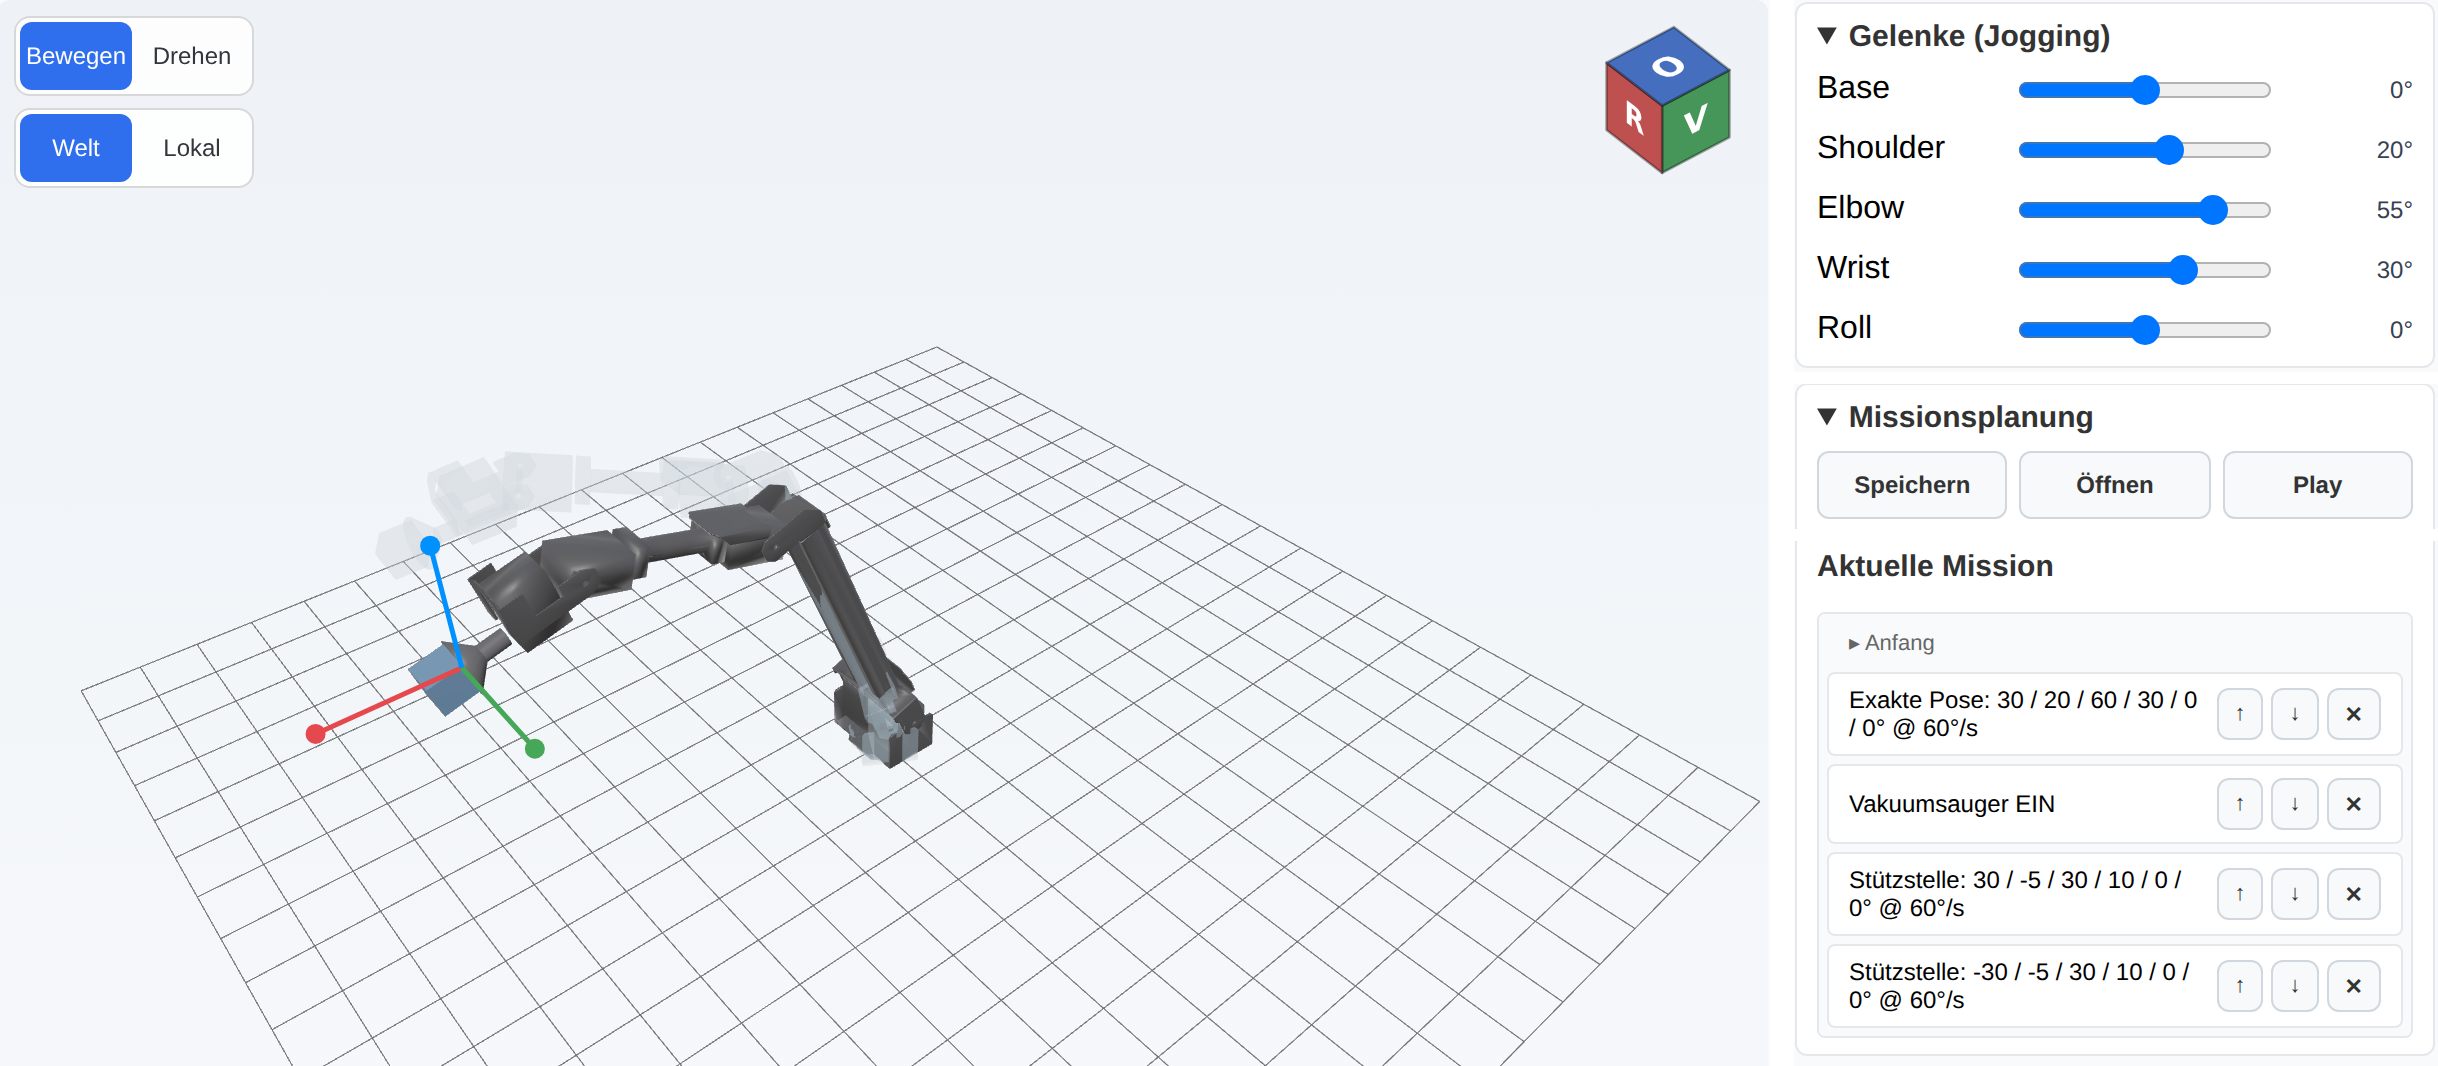
\includegraphics[width=0.75\linewidth]{fig3_teach_screenshots.png}
\caption{Missionsplanung (Ausschnitte): 3D-Modell mit Gizmo, ViewCube und Geisterbild; Gelenkschieber und Missionsliste.}
\label{fig:teach-screenshots}
\end{figure}


\section{Einsatz in der Lehre}

Die FCU soll in vier Lehrveranstaltungen eingesetzt werden (Tab.~\ref{tab:lehrveranstaltungen}), die alle an derselben greifbaren Anlage, jedoch an unterschiedlichen Schnittstellen ansetzen.

\begin{table}[htbp]
\centering
\small
\caption{Geplanter Einsatz der FCU in vier Lehrveranstaltungen.}
\label{tab:lehrveranstaltungen}
\begin{tabular}{p{0.20\linewidth}p{0.33\linewidth}p{0.37\linewidth}}
\toprule
\textbf{Veranstaltung} & \textbf{Lerninhalte} & \textbf{Nutzung der FCU und Aufgaben} \\
\midrule
Connected Systems (Master) & Kommunikationsgrundlagen, Signierung und Verschlüsselung in OPC UA, Echtzeitprotokoll EtherCAT & Modbus und OPC UA (Basic256Sha256, Sign, Gerätezertifikat) auf einem Prozessabbild; EtherCAT-Slave (LAN9253); Mitschnitte und Zertifikate untersuchen \\[2pt]
Regelungstechnik & Streckenidentifikation, Reglerentwurf, Anti-Windup & Druckregelstrecke: Kennlinie, Sprungantwort, Reglerbetrieb (P/PI/PID); Regler einstellen und vergleichen \\[2pt]
Automatisierungs\-technik & IEC 61131-3, Ablaufsprache (AS), Funktionsbausteinsprache (FBS) & Fabrik als reale Anlage; Soft-SPS (z.\,B. CODESYS) über OPC UA oder Modbus; Sortier- und Transportablauf, Inbetriebnahme \\[2pt]
Embedded Systems & Hardwarenaher Entwurf, Echtzeitbetriebssystem, Treiber & Modulare Platine, Testboard Nucleo-H563ZI, reproduzierbarer Build; Baugruppe oder Submodul weiterentwickeln \\
\bottomrule
\end{tabular}
\end{table}


\section{Evaluationsstand und geplante Weiterentwicklung}
\label{sec:evaluation}
Die grundlegende Funktion von Mechanik und Elektronik wurde im Rahmen studentischer Abschlussarbeiten nachgewiesen. Firmware und Build-Prozess sind implementiert und durch Unit-Tests abgesichert. Offen sind konkrete Aufgabenstellungen für alle Module sowie eine Befragung der Studierenden.

Zum Konferenzthema Energiemonitoring liefert der INA226 Spannung, Strom und Leistung der Anlage über alle Schnittstellen; in der Lehre lassen sich so Ablaufvarianten energetisch vergleichen. Für den Vollbeitrag soll dieses Energiemonitoring so erweitert werden, dass die Leistungsaufnahme den jeweils aktiven Verbrauchern verursachergerecht zugeordnet wird und sich der Energieverbrauch gezielt senken lässt. Darüber hinaus spart die FCU durch konsequent ressourceneffiziente Implementierungen Hilfsenergie in der Automatisierung ein: Weil Firmware, OPC-UA-Server und Web-UI schlank ausgelegt sind, genügt ein Mikrocontroller mit etwa 0,1\,W Leistungsaufnahme, wo sonst ein Mikroprozessorsystem mit mehreren Watt und aktiver Kühlung üblich ist. Der Web-Client lädt die Single-Page-Anwendung nur einmalig und tauscht danach ausschließlich kompakte Binärnachrichten per WebSocket aus, statt JSON-Strukturen zyklisch abzufragen. Synchrone Abwärtswandler anstelle asynchroner Wandler oder gar Linearregler senken die Verluste der Spannungsversorgung. Die Schrittmotortreiber passen den Spulenstrom per CoolStep lastabhängig an und senken ihn im Stillstand auf den minimal notwendigen Haltestrom ab; da er sich zur Laufzeit in weiten Grenzen softwareseitig einstellen lässt, wird er selbst zum Optimierungsgegenstand. Absolut betrachtet sind diese Einsparungen bei einer Modellfabrik selbstredend gering -- ihr eigentlicher Wert liegt darin, Studierende an einer greifbaren Anlage für den Energiebedarf scheinbar nebensächlicher Entwurfsentscheidungen zu sensibilisieren.

\section{Literatur}

\bibliographystyle{plain}
\bibliography{references}

\end{document}
